\documentclass{anstrans}

\usepackage{url}
\usepackage{subfigure}
%%%%%%%%%%%%%%%%%%%%%%%%%%%%%%%%%%%
\title{PyNE Progress Report} 
\author{Cameron~R.~Bates$^{1,2}$, Elliott~Biondo$^{3}$, Kathryn~Huff$^{2}$, 
Kalin Kiesling$^{3}$, Anthony~Scopatz$^{3}$ \\ 
 \hspace{1.0in}\\
Robert Carlsen$^{3}$,
Andrew Davis$^{3}$,
Matthew Gidden$^{3}$,
Tim Haines$^{3}$,
Joshua Howland$^{2}$,
Blake Huff$^{2}$,
Kevin Manalo$^{4}$,
Arielle Opotowsky$^{3}$,
Rachel Slaybaugh$^{2}$,
Eric Relson$^{3}$,
Paul Romano$^{5}$,
Patrick Shriwise$^{3}$,
John D. Xia$^{6}$,
Paul Wilson$^{3}$, and
Julie Zachman$^{3}$}

\institute{

$^{1}$ Lawrence Livermore National Laboratory, 7000 East Ave L-188, Livermore, CA 94550\\
\and $^{2}$ The University of California, Berkeley, 2521 Hearst Ave, Berkeley, CA 94709 \\
\and $^{3}$ The University of Wisconsin-Madison, 1415 Engineering Drive, Madison, WI 53706\\
\and $^{4}$ Georgia Institute of Technology, 770 State Street, Atlanta, GA 30332\\
\and $^{5}$ Massachusetts Institute of Technology, 77 Massachustts Avenue, Cambridge, MA 02139 \\
\and $^{6}$ University of Chicago, 5747 S. Ellis Ave., Jones 311, Chicago, IL 60637\\
}

\email{bates26@llnl.gov}

%%%% packages and definitions (optional)
\usepackage{graphicx} 

% allows inclusion of graphics
\usepackage{booktabs} 

% nice rules (thick lines) for tables
\usepackage{microtype} 

% improves typography for PDF
\newcommand{\SN}{S$_N$} 
\renewcommand{\vec}[1]{\bm{#1}} 

%vector is bold italic
\newcommand{\vd}{\bm{\cdot}} 

% slightly bold vector dot
\newcommand{\grad}{\vec{\nabla}} 

% gradient
\newcommand{\ud}{\mathop{}\!\mathrm{d}} 

% Common APIs
\newcommand{\Mesh}{\texttt{Mesh}} 
\newcommand{\Material}{\texttt{Material}} 

% upright derivative symbol
\begin{document}

%%%%%%%%%%%%%%%%%%%%%%%%%%%%%%%%%%%%%%%%%%%%%%%%%%%%%%%%%%%%%%%%%%%%%%%%%%%%%%%%
\section{Introduction}

PyNE is a suite of free and open source (BSD licensed) tools to aid in 
computational nuclear science and engineering. PyNE seeks to provide 
native implementations of common nuclear algorithms, as well as Python 
bindings and I/O support for industry standard nuclear codes. In the past 
year, the PyNE development team has improved PyNE's ease of use by making 
binaries available for Windows, Mac, and Linux through the conda package 
manager and adding Python 3 support. PyNE has also added many features 
including a Rigorous 2-step Activation workflow \cite{Biondo2014}, PyDAGMC 
integration, CADIS variance reduction, and expanded ENSDF parsing support. 
As a part of our ongoing efforts to implement a verification and validation 
framework we also added continuous integration using the Build and Test Lab 
at the University of Wisconsin.

\section{Usability Enhancements}
\subsection{Installation Improvements and Binary Distributions}
At our first PyNE workshop a significant amount of the instructional
time was devoted to PyNE installation and configuration. This reduced 
the amount of material we were able to cover significantly. From this
experience the PyNE development team came to the conclusion that a major
focus of our version 0.4 development efforts should be on making the 
installation process simpler for non-developers.
The core of this effort is based around the conda 
package manager. Conda is an open source package manager that is capable 
of managing packages on Windows, Mac and Linux. This makes it possible to use 
a single package manager across all platforms. We developed a standard conda 
package script which can be found at \url{https://github.com/conda/conda-recipes}. 
This automates the installation of dependencies for PyNE, significantly 
reducing the difficulty of building and installing the software.
In addition, we used this tool to produce binary 
packages on Linux and Mac. Finally, we developed a custom Windows build 
environment to build a distributable Windows binary.

\subsection{Python 3 Support}

PyNE was originally developed for the Python 2 interpreter as it was 
and still is the most common version of Python used in scientific computing. 
Python 3 is slowly starting to replace it, however, as the default Python 
version. With this changeover on the horizon the PyNE development team 
made an effort in preparation for the 0.4 release to make PyNE compatible 
with both versions. PyNE is now built and tested on Python 3 on a regular basis.

\section{Feature Enhancements}

\subsection{Mesh}

As of v0.4, PyNE includes a mesh representation interface that is used to 
build up geometries, store materials, and solve spatial differential equations.
This is implemented as a layer on top of MOAB meshes \cite{tautges_moab:_2004}.
In addition to the PyTAPS interface \cite{pytaps} it also adds PyNE materials to 
volume elements as well as a generic tagging interface. These features together 
form a generic, easy-to-use mesh library that is capable of handling a plethora
of nuclear engineering problems.

The \Mesh class lives in the \texttt{pyne.mesh} module. This class houses an 
iMesh instance called \texttt{mesh} which comes from PyTAPS and contains 
methods for native mesh operations. The \texttt{mats} attribute is an 
instance of a PyNE \texttt{MaterialLibrary}. This is a mapping of volume 
element handles to \Material objects. Tags---sometimes known as fields---are 
accessible as attributes on the mesh object itself. There are several different types
of tags (IMesh, Material, Metadata, Computed) depending on where the data should
be stored. All tag types expose the same interface. 

To do volumetric analysis and visualization, the \Mesh class is natively supported 
by the yt project \cite{2011ApJS..192....9T}. An example of the use of this mesh
to analyze nuetron flux in ITER is shown in Fig. \ref{ITER}

\begin{figure}
    \centering
    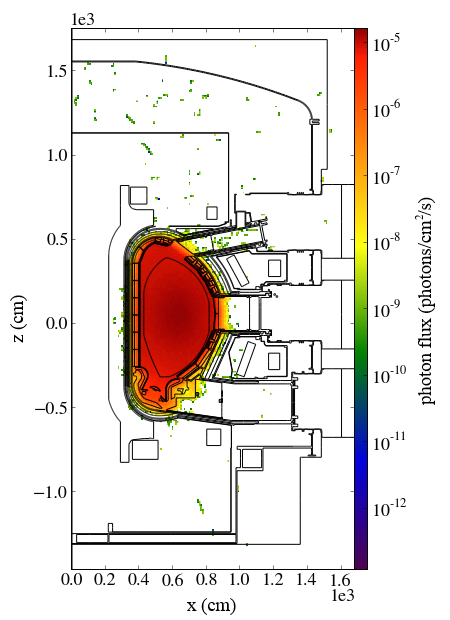
\includegraphics[width=7.1cm, angle =0]{iter_slice.png}
    \caption{A 2-D slice of a 3-D ITER flux mesh showing photon flux}
    \label{ITER}
\end{figure}


\subsection{PyDAGMC Integration}

Direct Accelerated Geometry Monte Carlo (DAGMC) is a component of MOAB that
facilitates Monte Carlo ray tracing on CAD geometries
\cite{tautges_acceleration_2009}.  A \texttt{dagmc} module has been added to
PyNE, providing a Python interface to these ray tracing capabilities. The
\texttt{dagmc.discretize\_geom()} function accomplishes the common task of
mapping geometry cells onto Cartesian or tetrahedral mesh. The
\texttt{cell\_fracs\_to\_mats} to method of the \texttt{Mesh} class can be used
to seamlessly create PyNE \texttt{Mesh} objects tagged with materials, where
the materials are mixtures of the contributions from the various geometry cells
found in each mesh volume element. This especially useful for discretizing CAD
geometries onto grids for deterministic methods. An example of this is shown in
Fig. \ref{mobius}.

\begin{figure}
\centering
\subfigure[CAD model of a complex geometry \cite{mobius}.]{
    \label{mobius_cad}
\hspace{1.3cm}
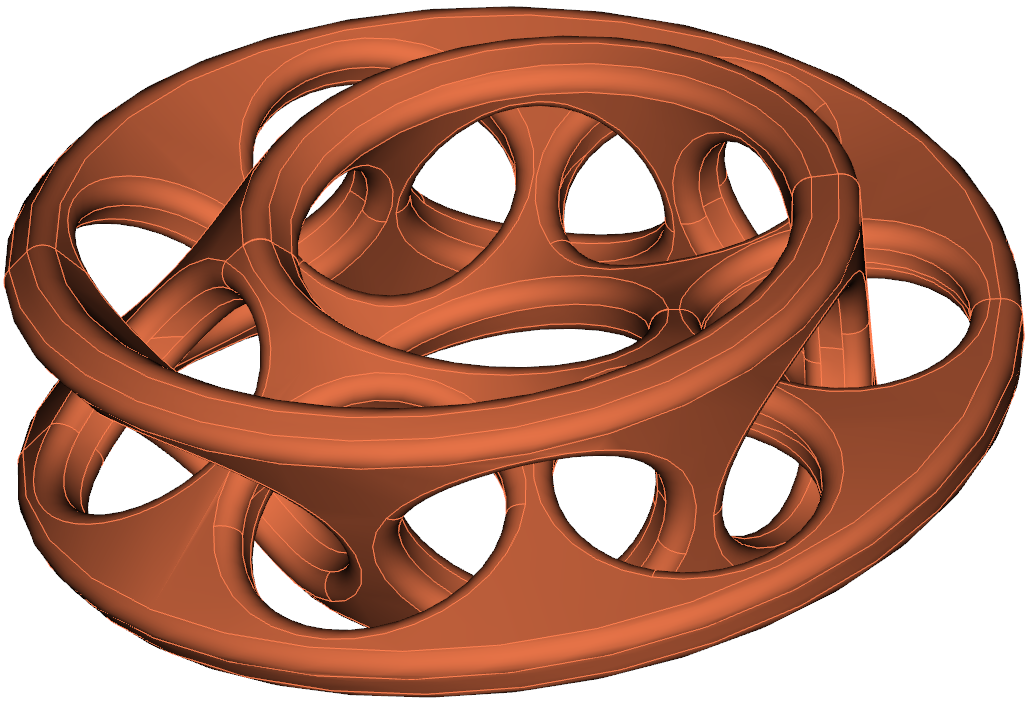
\includegraphics[width=5.86cm]{mobius_cad.png}
}
\subfigure[Volume fractions of the geometry within the mesh volume elements of an overlaid 200 x 100 x 200 Cartesian mesh.]{
    \label{mobius_mesh}
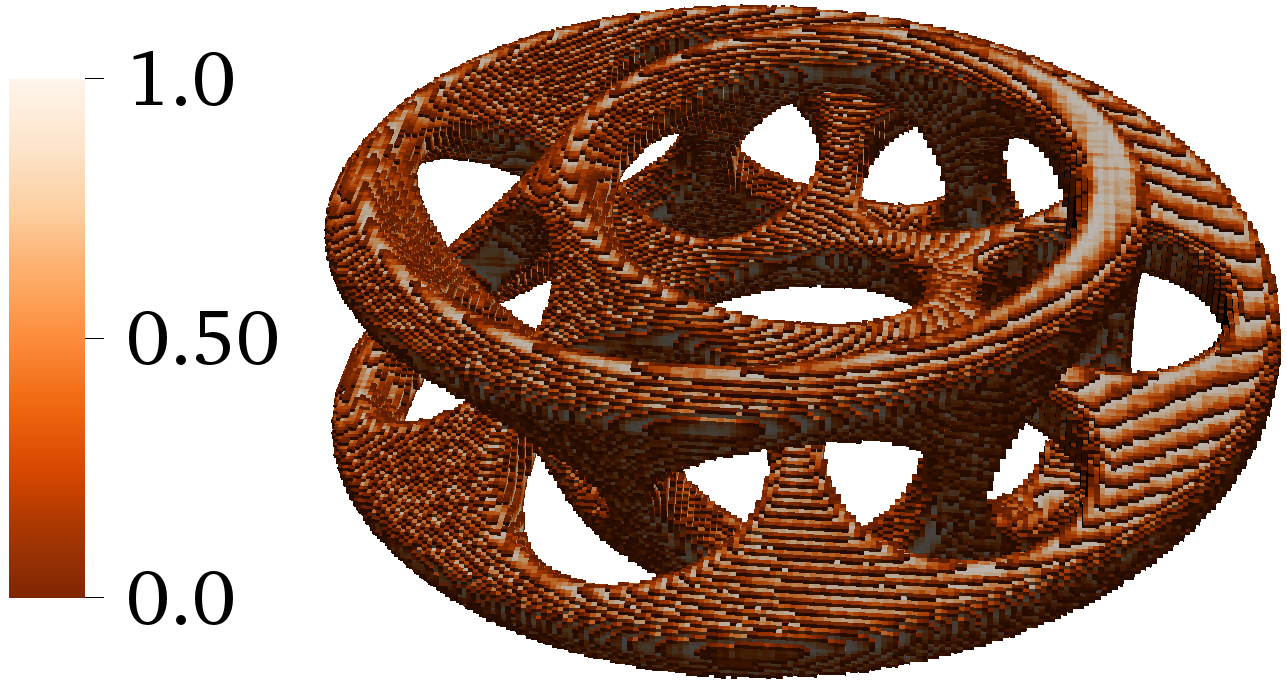
\includegraphics[width=7.5cm]{mobius_mesh.png}
}
\caption{A CAD geometry and a
discretized representation created using PyNE \texttt{discretize\_geom()}.}
\label{mobius}
\end{figure}


\subsection{ALARA Module}

ALARA is a nuclear inventory analysis code developed at University of Wisconsin
- Madison \cite{wilson_validation_1998}. A module has been added to generate
  ALARA input and parse ALARA output, primarily to and from PyNE \texttt{Mesh} objects. PyNE
\texttt{Mesh} objects tagged with flux and material data are used to generate
flux and material input. The compositions of activated materials as calculated by
ALARA can be read back into a PynE \texttt{Mesh} object. These components can be used
in mesh-based activation and burn-up workflows.

\subsection{R2S Activation Workflow}

The Rigorous Two-Step (R2S) method is used to estimate the shutdown dose rate
(SDDR) in fusion systems from photons born from neutron activation products
\cite{chen_rigorous_2002}. This method involves seperate neutron and photon
transport simulations, coupled to a dedicated nuclear inventory analysis code.
The PyNE \texttt{R2S} module impliments a mesh-based R2S method and
accomplishes this coupling in-memory by leveraging the PyNE \texttt{mesh},
\texttt{material}, \texttt{dagmc}, \texttt{mcnp}, and \texttt{alara} modules.
The \texttt{R2S} module currently only supports transport with MCNP and nuclear
inventory analysis with ALARA, but support for addtional physics codes is
planned. Mesh-based photon source sampling is accomplished within MCNP by
compiling MCNP against a custom source sampling library within PyNE.

% Not sure the best way to say this. Compile against pyne.so I guess? but it
% comes from source_sampling.cpp.

\subsection{CADIS Variance Reduction}

The Consistant Adjoint-Weighted Importance Sampling (CADIS) and the
Forward-Weighted CADIS (FW-CADIS) method are hybrid Monte Carlo variance reduction
techniques that use determinstic estimates of the forward and adjoint flux to
generate Monte Carlo weight windows and source biasing parameters
\cite{haghighat_monte_2003}. A mesh-based implimentation of this method has
been added to the PyNE \texttt{variancereduction} module. Work is currently
underway to interface with the Denovo \cite{Evans2010} deterministic transport
code to in order to acquire these determinsitic fluxes.


\subsection{Tally Class}

One common requirement in processing the output of MCNP and other nuclear
engineering codes is to keep track of multiple tallies. PyNE has added a
C++ class with a Python interface that assists users in keeping track of
tally data. The PyNE development team is working to add saving, loading,
and manipulation of these tally objects in the future.

\subsection{Fluka Module}

The \texttt{fluka} module is designed to parse the output files from FLUKA, a fully 
integrated particle physics Monte Carlo simulation package. Currently, 
this module only supports the parsing of USRBIN output files, which is 
a file similar to a meshtal file in MCNP in that it tracks a certain 
quantity over an evenly spaced volume mesh. This module parses the USRBIN 
files and saves the tracked data and percent error data as attributes of 
a mesh object.

\subsection{Amalgamation}

While PyNE is ostensibly a Python oriented toolkit over two-thirds 
of the codebase is written in C++. This makes it possible to use many 
of the features of PyNE without needing Python. In order to simplify 
the use of PyNE's C++ API we have added the ability to amalgamate all 
of the C++ code into a single source and header file. This makes it 
possible to add these two files to any project in order to use much of the 
functionality in PyNE without having to worry about linking multiple 
libraries in a seperate location. This is used in Cyclus (http://fuelcycle.org)
 to use PyNE features without adding a dependency on python.

\subsection{ENSDF Improvements}

Previous versions of PyNE have included some limited ENSDF parsing capabilities. 
These have been focused on extracting half lives and branching ratios of 
metastable and ground states. This has been vastly expanded to support the 
parsing of most ENSDF record types and to make level structure and decay data 
available in PyNE's C++/Python nuclear data interface. This makes it possible 
to use PyNE to look up most structure and decay data similar to online tools
such as NuDat. 

We have broken down the data from ENSDF into six distinct subsets. These 
include: excited level data, decay normalization data, gamma-ray data, alpha 
decay data, $\beta^-$ decay, and electron capture/$\beta^+$ decay. In addition 
to information about the radiations for all decay transitions listed in ENSDF we 
have also included atomic data from NNDC to calculate X-ray emmissions from 
conversion electrons in gamma ray emmission and electron capture/$\beta^+$ decay.
The combination of this data makes it possible to calculate coincidence rates for
gamma-rays.

\subsection{Fission Yield Data}

The latest release of PyNE includes two different sets of fission yield data. 
The first is the IAEA WIMSD library which provides fission product yields 
based on ENDF/B-VI. The second is from the IAEA Safeguards data library and includes 
independent fission yields with thermal, fast, and 14-MeV neutrons for $^{232}$Th, 
$^{233}$U, $^{235}$U, $^{239}$Pu, and $^{241}$Pu.

\section{Verification and Validation}

This issue will be addressed in more detail in other concurrent publications 
but the PyNE development team is working to implement documented verification 
and validation as a part of our basic development process. This has included: 
ensuring all code changes to PyNE have at least one reviewer who was not an 
author, requiring unit tests for all code additions, a coding style guide, 
and requiring all tests to pass on continuous integration builds before 
merging code changes. 


\section{Cultivation of Users and Developers} 
Computational toolkits in the sciences grow more robust by a broad user base who tests core capabilities with each use. Similarly, such toolkits grow more powerful by a broad developer base that serves the community by contributing new, research-relevant features. Development of a sustainable user and developer community is therefore integral to the success of the PyNE toolkit. To this end, the development team has organized tutorials to reach out to new users and has sought out support development by graduate students.

A tutorial at the University of California, Berkeley was organized in November to both reach out to new users and to gather feedback on the user experience of PyNE. Over a dozen researchers attended. The audience included undergraduate and graduate students in nuclear engineering as well as postdocs and faculty. In a six hour workshop, the attendees installed PyNE and ran prepared examples with the help of members of the development team. In addition to demonstrating the core data manipulation capabilities of the PyNE toolkit, the workshop included a reflective period in which attendees had the opportunity to brainstorm and suggest extensions, features, and improvements for the toolkit that were of interest in the context of their particular research.

Based on the success of this event and the organic growth of our user base, a second user workshop will be conducted at RPSD.

The development team has also conducted development sprints both UC Berkeley and the University of Wisconsin to cultivate the developer communities that have arisen in those institutions. These sprints allow the diverse and geographically dispersed development team to gather and collaborate on code contributions in a coherent manner.

In order to encourage young researchers to become involved in scientific computing, a number of desired PyNE extensions have been defined online. These short descriptions of desired extensions can be found on the PyNE website and are intended to guide the contributions of young researchers. By defining relevant independent contributions with realistic scope, these descriptions provide an opportunity for a beginner developer to contribute code in a guided manner and will assist their transition from user to developer.

\section{Conclusions}

In the past year the PyNE development team has worked to improve PyNE's 
usability in addition to adding new features. The availability of binaries 
for stable releases has made PyNE more accessible to those who are users 
but not developers. The PyNE project will continue to create free and open 
source tools that easily interface the plethora of choices available in 
nuclear engineering and scientific computing. 

%%%%%%%%%%%%%%%%%%%%%%%%%%%%%%%%%%%%%%%%%%%%%%%%%%%%%%%%%%%%%%%%%%%%%%%%%%%%%%%%
%%%%%%%%%%%%%%%%%%%%%%%%%%%%%%%%%%%%%%%%%%%%%%%%%%%%%%%%%%%%%%%%%%%%%%%%%%%%%%%%
\bibliographystyle{ans} 
\bibliography{bibliography} \end{document}
